% =========================================================================
% The Vent-Snap Ratchet — RA-L draft (target: RA-L submission ~Oct 2026)
% Build: pdflatex main && bibtex main && pdflatex main && pdflatex main
% (No local LaTeX on the dev box: compile on Overleaf with IEEEtran.)
% Status/TODO list: see paper/README.md. TODO markers render red inline.
% =========================================================================
\documentclass[journal]{IEEEtran}

\usepackage[utf8]{inputenc}
\usepackage[T1]{fontenc}
\usepackage{amsmath,amssymb}
\usepackage{graphicx}
\usepackage{booktabs}
\usepackage{multirow}
\usepackage{xcolor}
\usepackage[colorlinks=true,allcolors=blue!60!black]{hyperref}

% Draft TODO marker — strip before submission.
\newcommand{\TODO}[1]{\textcolor{red}{\textbf{[TODO: #1]}}}

% Convenience
\newcommand{\dstar}{\delta^{*}}
\newcommand{\kpa}[1]{$#1$\,kPa}

\begin{document}

\title{The Vent-Snap Ratchet: Quantifying, Modeling, and Eliminating
Seal-Rupture Slip in Suction-Based Wall Climbing Without Force Sensing}

\author{Shaopeng~\TODO{full author list, affiliations, funding}%
\thanks{Manuscript received \TODO{date}. This letter was recommended for
publication by \TODO{editor} upon evaluation of the reviewers' comments.}%
\thanks{The authors are with \TODO{affiliation}. Contact: \TODO{email}.}}

\markboth{IEEE Robotics and Automation Letters. Preprint version.}%
{Shaopeng \MakeLowercase{\textit{et al.}}: The Vent-Snap Ratchet}

\maketitle

% =========================================================================
\begin{abstract}
Legged robots that climb with vacuum suction cups must break a seal at
every step. On compliant, position-controlled platforms we show that this
seal rupture releases elastic energy stored in the leg chains: the body
drops within tens of milliseconds and the next adhesion locks the loss in
place, so that a robot stepping in place with zero net command descends by
a ratchet. Using a low-cost phone-video pipeline (normalized cross-correlation
tracking, per-run metric scale, command-marker time synchronization), we
quantify the effect at millimeter and per-leg resolution: $93\%$ of the
per-cycle position loss occurs within $100$\,ms of rupture, while during
venting itself the body is stationary---so slower venting provably
cannot help. A one-dimensional parallel-spring model explains the
loss and makes four predictions that we verify, including strict linearity
of the rupture bounce in a pre-laid unloading displacement. Building on
this, we propose the \emph{zero-force handover}: before venting, the
lifting leg's foot command walks back a per-leg calibrated displacement
$\delta_j$ while the supporting legs absorb it under a mean-invariant
apportionment with rotation-distance weights---purely kinematic, open
loop, and using no force, tactile, pressure, or current feedback. In an
$n{=}3$ Latin-square study the method cuts total slip by $43\%$
($\delta$ alone) and $61\%$ (with weights), and rupture-segment slip by
$82\%$/$88\%$ (paired $p\le0.0022$). A pre-registered rate-discrimination
experiment shows the residual transfer loss scales with laid millimeters,
not elapsed time ($\Delta b=\kappa\,\delta_j$, $\kappa$ reproduced to
$4\%$ across five days), identifying load-share allocation---not
speed---as the remaining lever ($\kappa$ reduced $44\%$ by the weights).
Data, logs, and the measurement pipeline are released.
\end{abstract}

\begin{IEEEkeywords}
Climbing robots, legged robots, compliance and impedance control,
calibration and identification, mechanism design.
\end{IEEEkeywords}

% =========================================================================
\section{Introduction}
\label{sec:intro}

\IEEEPARstart{L}{egged} climbing robots that adhere by vacuum must do
something wheeled and sliding-suction climbers avoid: at every single
step they destroy an adhesion contact and rebuild it elsewhere. For
negative-pressure feet the destruction is not gradual. A vented cup holds
its grip while residual vacuum persists and then lets go in one instant
when the seal lip peels---a \emph{rupture-type} detachment that
concentrates the mechanical consequences of releasing a loaded contact
into a few milliseconds, far below the control bandwidth of any gait
controller.

On a stiff robot this would matter little. But small wall-climbing
platforms are not stiff: safety margins are bought with lightweight,
3D-printed leg chains, bellows cups that conform to the surface, and
low-cost position-controlled servos with no torque feedback. On such a
platform we observed that a hexapod commanded to \emph{step in place} on
vertical glass---lift each foot and put it back exactly where it
was---slides down the wall by $57$--$74$\,mm per gait cycle, with zero
interfacial slip of the attached cups and zero drift at rest.
Frame-by-frame decomposition shows that in the $n{=}3$ study of this
letter $93\%$ of the loss occurs within $100$\,ms of seal rupture
($83\%$ in the initial discovery run, whose segmentation attributed more
to post-bounce re-equilibration), while during active venting, before
the seal lets go, the body moves less than $0.15$\,mm. The
mechanism is elastic: as the body sags, each attached leg chain is wound
up like a spring; venting a loaded leg cuts that spring at full tension,
the body falls until the remaining legs' additional deflection catches
it, and the next zero-preload adhesion locks the new position in. We call
the resulting staircase descent the \emph{vent-snap ratchet}. Servo
current corroborates the picture: bus current climbs step-wise from
$0.7$\,A to ${\sim}1.9$\,A over two cycles and does not relax---the legs
are increasingly fighting each other.

The failure combination---compliant support chains, rupture-type
detachment, and position-domain actuation that accumulates internal
forces \cite{gorner2009dlr}---is generic to low-cost suction climbers,
yet we found no prior quantification of the resulting whole-body position
loss (Sec.~\ref{sec:related}). Prior treatments of detachment disturbance
measure foot forces or body vibration and manage them with force sensors
in closed loop; the classical walking-machine literature unloads a leg
before lift-off entirely in the force domain. Our platform has no force,
tactile, or per-joint current sensing at all, and retrofitting it would
cost weight, wiring, and complexity precisely where climbing robots can
least afford them.

Instead we exploit the one fact that makes the problem tractable: an
attached foot cannot slip, so \emph{changing its position command changes
force, not position}. The unloading condition ``lift only a force-free
leg'' can therefore be translated from the force domain into the
displacement domain and executed open loop: before venting leg $j$, walk
its foot command back up-slope by a per-leg constant $\delta_j$---the
stored deflection, calibrated offline by linear extrapolation of the
rupture bounce---while the supporting feet absorb the same displacement
under weights that keep the six-leg command mean invariant, so the body
is commanded to stay put. We call this the \emph{zero-force handover}.

The contributions of this letter are:
\begin{enumerate}
\item \textbf{Discovery and quantification of the vent-snap ratchet.} To
the best of our knowledge, the first time-resolved, per-leg, millimeter
quantification of whole-body position loss at the instant of vacuum-seal
rupture in a legged suction climber, with a reproducible low-cost video
pipeline and released data. Prior reports of detachment disturbance are
qualitative for body motion, or quantify foot forces, accelerations, or
cavity pressure instead \cite{kim2008smooth,pei2023review,pan2005suction}.
\item \textbf{A parallel-spring account with verified predictions.} A
one-line elastic model explains the loss, predicts strict linearity of
the rupture bounce in the pre-laid displacement (verified; per-leg slopes
spread $4\times$ and furnish a stiffness estimate that agrees with an
independent route, $r=0.938$), predicts the dilution effect of load-share
weights ($-32\%$ predicted vs.\ $-31$--$33\%$ measured), and---via a
pre-registered discrimination experiment---yields a transfer-loss law
$\Delta b=\kappa\,\delta_j(1+0.20(r{-}1))$ in which time plays no role.
\item \textbf{A sensor-free, open-loop, software-only remedy with
$n{=}3$ evidence.} The zero-force handover converts pre-detachment
unloading---known in force-sensing closed-loop forms
\cite{cutkosky2010patent,nadan2024loris}---into the displacement domain:
offline per-leg calibration, mean-invariant apportionment, rotation
weights, no sensors of any kind in the loop. In a Latin-square $n{=}3$
study on glass it reduces total per-cycle slip by $43\%$/$61\%$ and
rupture-segment slip by $82\%$/$88\%$ (all pairwise comparisons
$p\le0.0022$, surviving Bonferroni correction).
\end{enumerate}

All claims of priority are made ``to the best of our knowledge'' and are
bounded carefully against the nearest prior work in
Sec.~\ref{sec:related}. Logs, videos, verification crops, and the
analysis pipeline will be released \TODO{package the open-data bundle;
add repository URL}.

% =========================================================================
\section{Related Work}
\label{sec:related}

\subsubsection{Platforms} Adhesive legged climbers divide by attachment
principle into vacuum/negative-pressure feet
\cite{hirose1991ninja,zhang2006sky,guan2013wclimbot,li2025biped},
dry/gecko-inspired adhesion \cite{unver2006geckobot,kim2008smooth,
henrey2014abigaille}, and grasping or spine-based feet
\cite{parness2017lemur,nadan2024loris}; see surveys
\cite{nansai2016survey,tao2023climbing}. This letter concerns the
oldest line, discrete-gait suction feet, where each step must break and
re-make a seal---a cost that sliding-suction designs
\cite{longo2004alicia,yue2024snail} avoid by paying for continuous
pumping instead. Our platform is a low-cost, 3-DOF-per-leg hexapod in
this lineage.

\subsubsection{Detachment disturbance: what has been measured} That
releasing an adhesive foot disturbs the rest of the robot is known
qualitatively: Stickybot's designers report that with isotropic pads the
large detachment force ``produc[ed] oscillations that frequently caused
the other feet to slip'' \cite{kim2008smooth}, and a recent Chinese
survey names ``transient and large detachment forces transmitted to the
trunk causing body shudder'' an open problem \cite{pei2023review}. What
has been \emph{quantified} is foot-level: peel-angle impedance control
reduces normal detachment force \cite{wang2021compliant}, rotational
peeling cuts pull-off force by $65.5\%$ \cite{wen2025force}, and
trajectory/force shaping reduces maximum detachment force by $28\%$ and
IMU-measured vibration by $82\%$ \cite{xiao2025ftfof}. We note explicitly
that the $82\%$ in \cite{xiao2025ftfof} is an acceleration amplitude
(m/s$^2$) and numerically coincides with, but is dimensionally unrelated
to, our $82\%$ reduction of rupture-segment \emph{displacement} (mm). In
the vacuum lineage the only transient quantification we found is of
cavity pressure \cite{pan2005suction}. Whole-body position loss per
detachment event---the quantity that actually bounds climbing
progress---appears in no prior work we could locate.

\subsubsection{Unloading before detachment} The idea of unloading a foot
before releasing it has force-domain, closed-loop precedents that we
must and do delimit against. The Stickybot patent describes tangentially
unloading a foot before lift-off to relax accumulated force and elastic
deformation, using Hall-effect force sensors in a stiffness-control loop
\cite{cutkosky2010patent}. LORIS's gait state machine contains an
explicit \emph{Unload} step that constrains the departing gripper's
contact force to zero in an online force optimization
\cite{nadan2024loris}. LEMUR~3 manages attach/detach forces with a
per-limb force sensor \cite{parness2017lemur}; admittance control
mitigates reaction forces on limbed climbers in simulation
\cite{imai2024admittance}; reaction-aware planning shapes swing inertia
\cite{ribeiro2023ramp}; quasi-static gait optimization redistributes
contact forces at the planning level \cite{boscariol2013optimal}.
All of these execute in the force domain, in closed loop, or at the
planning layer, and none quantifies body slip. Our claim is accordingly
narrow: converting the unloading condition to the \emph{displacement
domain} (per-leg offline calibration, mean-invariant apportionment),
executing it \emph{open loop on a platform with no force sensing
whatsoever}, and validating it by \emph{rupture-segment slip}.

\subsubsection{Force distribution in walking machines} Smoothly driving
a leg's force to zero before lift-off is a classical walking-machine
topic from Waldron's force/motion management onward
\cite{waldron1986force,kumar1988force,klein1990optimal,zhou2000fricom,
erden2007torque}, through to modern whole-body controllers and MPC
\cite{righetti2013optimal,bellicoso2016perception,focchi2017high,
dicarlo2018dynamic}. The entire line executes in the force domain: either
force/torque sensors close the loop \cite{gorinevsky1990force,
gorner2009dlr}, or force setpoints are handed to actuators that can track
them. Chen et al.'s ``does not require force sensors''
\cite{chen1999optimal} refers to the setpoint computation only. The DLR
Crawler paper states the problem we start from---position-controlled
multi-legged robots accumulate internal forces---and solves it with joint
torque sensing \cite{gorner2009dlr}. Insects solve it too: load transfer
to neighboring legs mechanically unloads a leg, and load sensors trigger
its swing \cite{dallmann2017load}---a biological closed loop that our
open-loop table replaces. In this classical frame, our contribution is a
new execution domain for an old requirement, on a platform class (hobby
position servos, strong series compliance) the classical solutions do
not cover.

\subsubsection{Displacement-domain feed-forward for compliance}
Calibrate-then-feed-forward compensation of structural compliance is
itself a mature method family: TITAN~XI pre-calibrates leg flexibility to
restore foothold accuracy on slopes \cite{doi2005titan}; Ota et al.\
compensate gravity-induced deformation on a suction quadruped for motion
smoothness \cite{ota2006deformation}; machining robots correct commanded
trajectories from offline stiffness models \cite{wang2009machining,
klimchik2014compliance}; legged humanoids feed forward sole/joint
deformation \cite{takenaka2005floor}; a gecko-inspired climber applies
stiffness-model-based gravity compensation for posture
\cite{wang2024gecko}; sway compensation shifts the body to transfer
\emph{gravity} load in static gaits \cite{kurazume2002feedforward}. Same
mathematical shape, different target: none of these uses calibrated
displacement to \emph{zero the internal force of a leg about to
detach}, and none faces energy release concentrated into milliseconds.

\subsubsection{Alternative routes} One can avoid rupture altogether
(sliding suction \cite{yue2024snail}, at the price of continuous power),
estimate contact force from motor current \cite{wahrburg2018motor}
(infeasible on hobby servos with large gearbox friction; see
Sec.~\ref{sec:discussion}), or exploit snap-through energy release for
propulsion instead of suffering it \cite{tang2020spine}---the same
physics used in the opposite direction. Directional dry adhesives detach
at near-zero force by material design \cite{kim2008smooth,
autumn2006frictional}; vacuum cups cannot inherit that trick, which is
precisely why the stored energy must be \emph{returned before rupture}.
Slow venting, the intuitive remedy, is refuted by our data
(Sec.~\ref{sec:phenomenon}).

% =========================================================================
\section{Platform, Pipeline, and the Phenomenon}
\label{sec:phenomenon}

\subsection{Platform}
\label{sec:platform}

The testbed (Fig.~\ref{fig:platform}) is a 3D-printed hexapod derived
from an open-source walking platform, with self-designed suction feet:
each 3-DOF leg (coxa/femur/tibia $43/80/124$\,mm) ends in a 30\,mm
bellows suction cup fed through a normally-closed 3-way solenoid valve
and a per-foot check valve. Two diaphragm pumps hold the attached cups
between $-60$ and $-75$\,kPa by bang-bang hysteresis; adhesion is
declared below $-30$\,kPa; a leg may lift only when the five other cups
are attached and deeper than a $-50$\,kPa gate. Eighteen 35\,kg$\cdot$cm
position-controlled hobby servos (no torque, force, tactile, or
per-joint current feedback of any kind) are driven by a Raspberry~Pi~5
through an RP2040 servo board; total mass is ${\sim}2.7$\,kg
\TODO{final weigh-in of assembled robot}. All experiments run on
vertical glass with a safety rope. The platform's compliance is not
incidental: printed legs, bellows cups, and servo gear trains together
make the body-to-anchor chain soft enough that commanded body motion is
only $42\%$ realized (Sec.~\ref{sec:finding2})---typical of the
lightweight construction this robot class requires.

\begin{figure}[t]
\centering
\fbox{\parbox[c][4.2cm][c]{0.95\linewidth}{\centering
\TODO{Fig.~1: (a) robot on glass wall, (b) leg chain schematic with
compliance sources and suction foot cutaway, (c) handover kinematics
sketch (lifting leg walks back $\delta_j$ up-slope, supports absorb
$w_i\delta_j$ down-slope).}}}
\caption{Platform and the zero-force handover.}
\label{fig:platform}
\end{figure}

\subsection{Measurement pipeline}
\label{sec:pipeline}

We measure body position along the wall from a fixed phone camera
(4K@30\,fps) by normalized cross-correlation (NCC) template tracking of
the robot's electronics board, with sub-pixel parabolic interpolation and
frame-wise compensation of camera motion against a static reference
patch. Metric scale is taken \emph{per run} from the long edge
(93.0\,mm) of a PCB rigidly mounted on the robot, localized by
four-corner sub-pixel fits ($0.288$--$0.296$\,mm/px across runs;
top/bottom edge disagreement $0.2$--$1.9\%$). Video time is registered
to the robot's on-board event log by a commanded time-sync marker: a
$\pm10$\,mm body lean executed at the start of each run and fit in shape
to the tracked trajectory ($R^2$ $0.95$--$1.00$ per run); the same
marker doubles as a compliance probe (Sec.~\ref{sec:finding2}). Every
lift event is then decomposed into \emph{handover} (displacement laying,
when enabled), \emph{vent} (a fixed $[-1,+0.4]$\,s window around the
logged pressure-zero event, containing the seal rupture), \emph{swing},
\emph{press} (touchdown), and \emph{settle} segments. The pipeline was verified against a manual tape-ruler reading
($131$\,mm total vs.\ $131.3$\,mm tracked) and 188 archived localization
crops; all scale boards and template locks were human-checked
\TODO{exact vent-window definition: confirm $-1$\,s/$+0.4$\,s bounds
from ab\_quant before submission}.

\subsection{The vent-snap ratchet}
\label{sec:ratchet}

Stepping in place is the cleanest probe: each leg in the fixed rotation
order (R3$\to$L1$\to$R2$\to$L3$\to$R1$\to$L2) is lifted $33$\,mm,
hovers $1$\,s, and is put back at exactly its former station; the
commanded net body motion is zero, so any systematic displacement must
come from elastic strain release and re-locking. Two controls verify the
premises: ink marks on the glass beside each attached cup do not move
(zero interfacial slip), and the body is stationary during all-feet
attached dwell (zero time-type creep; see also
Sec.~\ref{sec:mechanism}). Yet the body descends $57$--$74$\,mm per cycle
(discovery run; $63.9\pm0.9$\,mm in the $n{=}3$ baseline,
Sec.~\ref{sec:results}), in a staircase whose every step coincides with
a seal rupture (Fig.~\ref{fig:staircase}).

\begin{figure}[t]
\centering
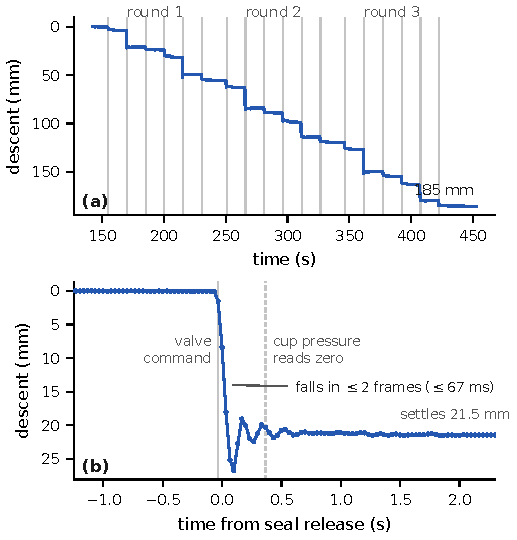
\includegraphics[width=\linewidth]{figures/fig_staircase_zoom.pdf}
\caption{The vent-snap ratchet (baseline, replication \#1).
(a)~Body position along the wall over three rounds of stepping in
place: every step of the $185$\,mm staircase coincides with a seal
rupture (gray lines); the trace is flat between events.
(b)~Native-30\,fps profile of one lift (L1, round 2), $t{=}0$ at the
tracked release: the body is stationary before the release, falls
$21.5$\,mm within two frames with an underdamped overshoot (peak
$26.7$\,mm); the released foot simultaneously recoils $12.8$\,mm
down-wall (not shown). The logged valve command and pressure-zero
events bracket the mechanical release; their placement relative to the
video carries the sync uncertainty (a few tenths of a second).}
\label{fig:staircase}
\end{figure}

Three time scales matter. (i)~While residual vacuum drains after the
venting command, the body does not move ($<0.15$\,mm). (ii)~At seal
rupture the entire drop completes within $1$--$2$ frames
($33$--$67$\,ms), with an underdamped overshoot (L1: peak $23.8$\,mm,
settle $21.5$\,mm)---a textbook elastic release. (iii)~Between events
the trajectory is flat. In the $n{=}3$ baseline the vent segments sum to
$172.9\pm3.4$ of $185.5\pm3.0$\,mm total---$93\%$; touchdown press
contributes $4\%$ (discovery-run decomposition: $83\%$/$4\%$ with wider
re-equilibration windows). The released foot itself recoils
$9$--$15$\,mm down-wall at the same instant. Per-leg single-event
bounces reach $20.9$\,mm (L1) and $19.2$\,mm (R1)---the top (front)
legs, where peel moments concentrate---versus $5.8$\,mm for the softest
legs, a first sign that leg-chain stiffness is strongly unequal.

Two corollaries fix the design space. First, \emph{slow venting cannot
work}: the force release is not distributed over the pressure decay but
compressed into the lip's peel instant; the data show zero motion while
residual vacuum drains. Any remedy must ensure the leg carries no force
\emph{at the moment the seal lets go}. Second, the loss is locked in by
the next adhesion: a fresh cup grips wherever the body then hangs, at
zero preload (Sec.~\ref{sec:model}), so the drops accumulate as a
ratchet rather than averaging out. Servo bus current tells the same
story electrically: from $0.73$\,A at first attachment it climbs
step-wise to ${\sim}1.9$\,A after two cycles and does not relax---each
locked-in drop leaves the support legs fighting a larger internal force.

% =========================================================================
\section{A Parallel-Spring Account}
\label{sec:model}

\subsection{Model}

Collapse each attached leg chain $i$ to a linear spring of stiffness
$k_i$ along the wall's gravity axis ($x$ positive down). Let $a_i$ be
the (immovable) anchor of foot $i$ and $c_i$ its commanded position in
the body frame, and define $y_i \equiv a_i - c_i$: the body position at
which leg $i$ would carry zero force. Leg $i$ then exerts the shear
force $f_i = k_i\,(x - y_i)$ on the body (positive up-wall), and static
equilibrium of the attached set $S$ gives
\begin{equation}
x \;=\; \langle y\rangle_k + \frac{mg}{K},
\qquad
\langle y\rangle_k \equiv \frac{\sum_{i\in S} k_i y_i}{K},\;\;
K \equiv \sum_{i\in S} k_i .
\label{eq:equilibrium}
\end{equation}
The body hangs below the \emph{stiffness-weighted} mean of the legs'
zero-force positions. Three events drive the dynamics:

\emph{Zero-preload lock-in.} A cup that seals grips wherever the body
currently is, storing no force: adhesion sets $y_j \leftarrow x$.

\emph{Rupture.} Venting leg $j$ removes a spring carrying tension
$f_j$; the body falls to the new equilibrium of the catching set,
\begin{equation}
b_j \;=\; \frac{f_j}{K - k_j},
\label{eq:bounce}
\end{equation}
i.e.\ \emph{the observed bounce is the leg's stored force divided by the
parallel stiffness of the other legs}---not the leg's own stored
deflection $e_j = f_j/k_j$. The ratio $e_j/b_j = (K-k_j)/k_j$ is
$5$--$8$ on our platform, a distinction that matters for calibration
(Sec.~\ref{sec:calib}).

\emph{Winding.} Between adhesion and lift, every millimeter the body
descends winds each attached leg by one millimeter ($x-y_i$ grows);
older anchors are wound tighter, so the legs' stored forces differ even
under identical commands.

Iterating lock-in, winding, and rupture over the gait reproduces the
ratchet: in the 1-D simulation the steady-state in-place loss is
${\approx}0.4\,mg/\bar{k}$ per cycle, and matching the observed
$74$\,mm/cycle gives a whole-robot compliance scale of
$mg/\bar{k}\approx185$\,mm. The measured single-event bounce saturates
near $21$\,mm, below the linear prediction---servo torque saturation
caps the energy a single leg can store, which also explains why forward
climbing still nets $+26\%$ of commanded stride rather than losing
ground \TODO{net-advance demo (T4b) will refresh this number}.

\subsection{Four verified predictions}
\label{sec:predictions}

\emph{P1: The rupture bounce is strictly linear in a pre-laid unloading
displacement, with slope encoding leg stiffness.} If, before venting,
$y_j$ is walked toward $x$ by $\delta$ (Sec.~\ref{sec:method}), the
residual tension falls by $k_j\delta$, so
$b_j(\delta) = b_j(0) - s_j\,\delta$ with
$s_j = k_j/(K-k_j)$. A three-dose calibration experiment
($\delta = 0/12/24$\,mm uniform; Sec.~\ref{sec:calib},
Fig.~\ref{fig:linearity}) finds all six legs strictly linear (mid-dose
residual $\le1$\,mm), with slopes $0.13$--$0.57$---a $4\times$ per-leg
spread that directly measures the stiffness imbalance. The normalized
stiffnesses $\hat{k}_j = s_j/(1+s_j)$ from these slopes agree with a
completely independent second route (fitting handover-segment sag,
Sec.~\ref{sec:mechanism}) at Pearson $r=0.938$.

\emph{P2: A freshly attached leg bounces by nothing.} Zero-preload
lock-in implies the first lift of a just-attached leg releases only the
force accrued since lock-in: measured first-round first-lift bounces are
${\approx}0$ ($-0.0$ and $+1.8$\,mm in two independent runs), rising in
later rounds as winding accumulates.

\emph{P3: Equilibrium is stiffness-weighted, so mean-invariant commands
do not perfectly freeze the body.} By \eqref{eq:equilibrium}, a
handover that moves $y_j$ up by $\delta$ and the supports down by
weights $w_i$ ($\sum w_i = 1$) shifts equilibrium by
\begin{equation}
\Delta x \;=\; \frac{\delta\,\bigl(k_j - \sum_{i\in S\setminus j} k_i
w_i\bigr)}{K},
\label{eq:redistribution}
\end{equation}
zero only for equal stiffness. Unloading the \emph{stiffest} leg must
sink the body; the first-order prediction for L1 is $4.6$\,mm vs.\
$6.8$\,mm measured (first round), and the full fitted form of
\eqref{eq:redistribution} reproduces all $18$ leg$\times$round cells of
the B condition with RMSE $0.85$\,mm (Sec.~\ref{sec:mechanism}).

\emph{P4: Load-share weighting dilutes stored energy non-monotonically.}
Because each lock-in re-zeros one leg, load handed to a support early is
partially re-absorbed by subsequent lock-ins, while load handed late is
carried intact into that leg's own lift. Weighting the handover shares
toward the legs \emph{farthest from their next lift} (most dilution
opportunities ahead) lowers steady-state stored energy: the 1-D model
gives $-19\%$ (mild), $-32\%$ (the deployed schedule
$0.6/0.25/0.1/0.05/0$), $0\%$ (all-to-one; non-monotonic), and $+30\%$
(reversed---worse than uniform). The measured B$\to$C reduction of
residual slip is $-31$--$33\%$ across metrics
(Sec.~\ref{sec:results}).

\begin{figure}[t]
\centering
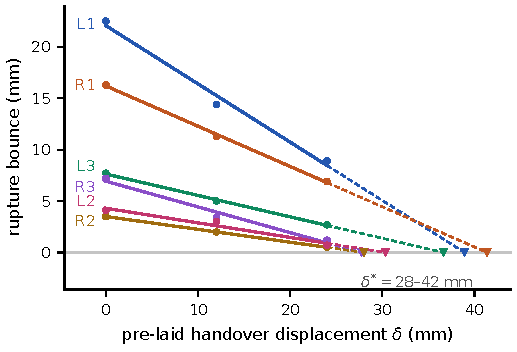
\includegraphics[width=\linewidth]{figures/fig_bounce_delta.pdf}
\caption{P1 verified: rupture bounce vs.\ pre-laid displacement
$\delta$ (round 2 of the three-dose calibration, $\delta=0/12/24$\,mm
uniform). All six legs are strictly linear (mid-dose residual
$\le1$\,mm); the slopes spread $4\times$ across legs (stiffness
imbalance), and the dashed extrapolations to zero bounce define the
calibration targets $\dstar_j=28$--$42$\,mm (triangles).}
\label{fig:linearity}
\end{figure}

% =========================================================================
\section{Zero-Force Handover}
\label{sec:method}

\subsection{Displacement-domain unloading}

The remedy follows from one invariant: an attached cup does not slip
(verified, Sec.~\ref{sec:ratchet}), so foot commands move forces, not
feet. Before venting leg $j$, the gait engine inserts a HANDOVER phase:
the lifting leg's foot command walks \emph{up-slope} by $\delta_j$
(returning its stored deflection), while each supporting foot command
walks \emph{down-slope} by $w_i\,\delta_j$ with $\sum_{i} w_i = 1$
(absorbing the load), both laid quasi-statically at $10$\,mm/s along the
gravity direction maintained by the engine. The six-command mean is
invariant, so the body is commanded to stay put; the lifted leg's force
is walked to zero; the seal then ruptures with nothing to release. The
supports never carry more than they would carry \emph{after} the lift
anyway---the handover only moves the transfer earlier and makes it
lossless. Commands remain bounded: over one gait cycle a support absorbs
${\approx}\delta$ down-slope in shares and returns $+\delta_j$ when its
own turn comes, so offsets do not diverge (with per-leg tables the
touchdown reset absorbs the small residual; the first-round command
artifact this causes is bounded at ${\sim}5$\,mm and vanishes in steady
state).

\subsection{Per-leg calibration: bounce is not stored energy}
\label{sec:calib}

The naive calibration---set $\delta_j$ to the observed bounce---fails
by the factor in \eqref{eq:bounce}: the bounce is the stored force read
through the \emph{other} legs' parallel stiffness, and underestimates
the stored deflection $5$--$8\times$. (Our first table, bounce
$\times0.8$, reduced per-cycle slip only $74\to50$\,mm at full dose.)
The correct, scale-free procedure drops out of P1: run three doses
($\delta = 0$, half, full), fit the per-leg line, and extrapolate to the
zero-bounce intercept $\dstar_j = b_j(0)/s_j$. Measured
$\dstar = 28$--$42$\,mm per leg; we deploy $\delta_j = 0.8\,\dstar_j$
(under-shoot discipline: a small residual bounce is benign, overshooting
pre-loads the leg in reverse), giving the table
L1/R1/L3/R3/R2/L2 $= 31/33/29/22/22/24$\,mm. Because $\dstar$ is a
ratio of same-unit quantities, it is independent of the video scale
calibration---the most robust number in this letter. Doses respond
cleanly ($65.6\to50.0\to38.7$\,mm per cycle across $0/12/24$), and the
staircase character is unchanged: $\delta$ lowers each step's height,
not its timing.

\subsection{Rotation-distance load-share weights}

P4 fixes the apportionment: shares are assigned by \emph{rotation
distance}---the support that just lifted (farthest from its next lift)
receives the largest share, the next-to-lift receives none
($0.6/0.25/0.1/0.05/0$ in rotation order). The engine re-normalizes over
the current support set each tick and falls back to uniform shares (with
a logged note) if the lift order ever deviates from the rotation---the
weights assume the cyclic gait, and misapplying them would pile load
onto one leg. Weights change the steady-state operating point, so the
$\delta$ table is calibrated \emph{under} the weight schedule
(Sec.~\ref{sec:protocol}).

\subsection{Implementation and guards}

The method is ${\sim}200$ lines in the gait engine: one new phase
between the lift decision and VENT, one per-tick displacement update, no
new hardware, no sensing, no per-robot tuning beyond the $\delta$ table.
Safety guards (none of which fired in any run reported here): the laying
pauses during leak-rescue; every per-tick target is envelope-checked and
the handover is truncated (partial unloading, logged) rather than
driving a support out of workspace; and the $-50$\,kPa lift gate is
re-checked after laying, since seconds have passed since the lift
decision. Handover adds $\delta_j/10$\,mm/s $\approx2.2$--$3.3$\,s per
step at the deployed table---the price in cycle time; the energy price
is quantified in Sec.~\ref{sec:cost}.

% =========================================================================
\section{Experiments}
\label{sec:experiments}

\subsection{Protocol}
\label{sec:protocol}

\emph{Conditions.} A: baseline stepping in place; B: A $+$ zero-force
handover with the calibrated table ($\delta_j = 0.8\dstar_j$); C: B $+$
rotation-distance weights (table calibrated under weights). One variable
changes per condition.

\emph{Design.} $n{=}3$ full-protocol replications, each an independent
mount--run--dismount of all three conditions, ordered by a $3\times3$
Latin square (\#1 A$\to$B$\to$C, \#2 B$\to$C$\to$A, \#3 C$\to$A$\to$B)
so that condition is decoupled from within-session order, battery
state, and glass condition. Each run: one keypress launches a fixed
automated sequence---$60$\,s settle, $\pm10$\,mm time-sync marker,
then $3$ rounds $\times$ $6$ legs of lift--hover--replace with
pressure-gated pacing (next lift waits for pump-off at $-75$\,kPa),
$15$\,s between rounds, $30$\,s final settle---so pacing is identical
across runs by construction. Battery $\ge7.9$\,V at each session start;
camera untouched within a session; scale re-measured per run. All nine
logs show zero freezes, zero envelope truncations, zero gate waits.
Judgment uses round 2 by protocol (round 1 contains the known ramp-up
and command-reset artifacts; round 3 is the replicate check).

\subsection{Main results}
\label{sec:results}

\begin{table}[t]
\caption{Main results, $n{=}3$ Latin square (mm; mean $\pm$ sample SD
over replications). Percentages vs.\ A.}
\label{tab:main}
\centering
\footnotesize
\setlength{\tabcolsep}{3.5pt}
\begin{tabular}{@{}lrrr@{}}
\toprule
 & A (baseline) & B ($+\delta$) & C ($+$weights) \\
\midrule
Round-2 slip & $63.9\pm0.9$ & $38.1\pm1.0$ & $26.5\pm1.7$ \\
3-round total & $185.5\pm3.0$ & $105.6\pm2.2$ & $72.9\pm3.0$ \\
 & & $(-43\%)$ & $(-61\%)$ \\
Rupture segment & $172.9\pm3.4$ & $31.6\pm1.0$ & $20.1\pm3.3$ \\
 & & $(-82\%)$ & $(-88\%)$ \\
Handover segment & --- & $60.2\pm2.2$ & $39.7\pm4.3$ \\
Current rise (A) & $+0.97\pm0.02$ & $+2.40\pm0.08$ & $+1.85\pm0.08$ \\
\bottomrule
\end{tabular}
\end{table}

Table~\ref{tab:main} and Fig.~\ref{fig:waterfall} are the headline.
Paired per-replication
differences (df $=2$, two-sided): B$-$A $=-79.9\pm5.0$\,mm
($t=27.9$, $p=0.0013$); C$-$A $=-112.6\pm5.9$\,mm ($t=32.9$,
$p=0.00092$); C$-$B $=-32.7\pm2.7$\,mm ($t=21.4$, $p=0.0022$). All
three survive Bonferroni correction for the three comparisons
($p\times3 < 0.007$). We emphasize what $n{=}3$ means here: three
\emph{full-protocol} independent replications, each containing
$18$ lift events per condition, with relative effects nearly constant
across replications (B/A: $-42/-45/-42\%$; C/A: $-61/-63/-58\%$)---the
treatment effect is an order of magnitude larger than every noise scale
in the experiment. No order effect is visible after the Latin-square
decoupling.

Per-leg rupture bounces (round 2, $n{=}3$): the baseline reproduces the
discovery run five days earlier (A-condition L1 $20.1\pm1.3$ vs.\
$20.9$); under C all legs are ${\le}2.4$\,mm, and the stiff front legs
that dominated the baseline are $0.9\pm0.5$ (L1) and $0.9\pm0.3$\,mm
(R1)---a $95\%$ per-leg reduction where it mattered most. R1 showed
occasional slight upward bounce ($-1$ to $-3$\,mm), the signature of
mild overshoot, accepted per the under-shoot discipline.

\begin{figure}[t]
\centering
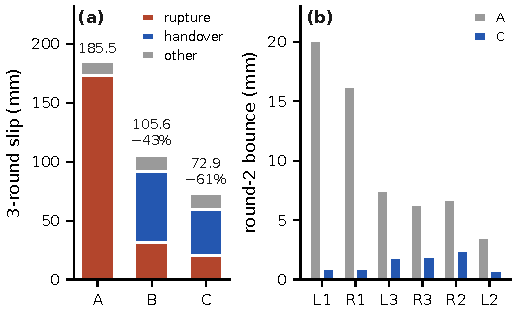
\includegraphics[width=\linewidth]{figures/fig_waterfall.pdf}
\caption{Where the loss lives ($n{=}3$ means). (a)~Three-round slip by
segment and condition: the handover converts an impulsive $173$\,mm
rupture loss into a $60$\,mm quasi-static transfer loss; weights
compress it to $40$\,mm. (b)~Per-leg round-2 rupture bounce, A vs.\ C:
the stiff front legs drop from $20.1$/$16.2$ to $0.9$/$0.9$\,mm.}
\label{fig:waterfall}
\end{figure}

\subsection{Finding 1: the residual lives in the transfer, on the
stiffest legs, and grows}
\label{sec:finding1}

With rupture slip suppressed, $56$--$62\%$ of the B/C residual sits in
the \emph{handover segments}, concentrated on the two stiffest legs and
growing round over round (B-condition L1: $6.8\to10.3\to12.6$,
$6.9\to8.6\to10.6$, $6.7\to8.8\to11.9$\,mm across the three
replications; R1 similar; the other four legs $0$--$1.5$\,mm). The
first-order reading---P3's stiffness-weighted equilibrium---is correct
about the \emph{shape} but, as the modeling below shows, wrong about the
\emph{size}: redistribution explains only ${\sim}7$\,mm of the
$60$\,mm segment. The decomposition of this residual, and which lever
actually moves it, is the subject of Sec.~\ref{sec:mechanism}.

\subsection{Finding 2: a $42\%$ command-to-body transfer ratio}
\label{sec:finding2}

The $\pm10$\,mm time-sync marker doubles as a compliance probe: across
$9$ markers, $3$ days, and $3$ camera setups, the commanded $10$\,mm
body lean produces $4.22\pm0.30$\,mm of actual body motion---a
\emph{transfer ratio of $42.2\pm3.0\%$}, invariant across conditions
(A/B/C $4.15/4.28/4.22$\,mm), as expected for a probe executed at full
static support. Sixty percent of commanded displacement is absorbed by
the leg chains. We report this as a platform characterization, not new
physics: it quantifies the compliance that makes the ratchet large, and
it feeds the model's overall gain (the fitted $c_0$ below).

\subsection{Mechanism: fits, and a pre-registered discrimination
experiment}
\label{sec:mechanism}

\subsubsection{Fitting the handover segment}
Per-leg, per-round handover-segment displacements (B: $54$ cells over
$3$ replications) are fit by
\begin{equation}
\Delta b_{j,r} \;=\;
c_0\,\delta_j\bigl(\hat{k}_j - \textstyle\sum_i \hat{k}_i s_i\bigr)
\bigl(1+\gamma(r{-}1)\bigr) \;+\; \Delta b^{\mathrm{cm}}_{j,r},
\label{eq:fit}
\end{equation}
the first term being \eqref{eq:redistribution} with a round-growth
factor $\gamma$ and the second a \emph{common-mode} term shared by all
legs. Within B, the model achieves RMSE $0.85$\,mm on signals of
$6.8$--$12.6$\,mm with leave-one-replication-out CV of $0.99$\,mm, and
the fitted $\hat{k}$ agrees with the slope route of P1 at $r=0.938$
(final joint estimate: L1 $0.265$, R1 $0.227$, L3 $0.137$, R2 $0.133$,
R3 $0.125$, L2 $0.112$; $\gamma=0.11$). The account it returns is a
reversal of the first-order reading: B's $60.2$\,mm segment $=$
${\sim}6.7$ redistribution $+$ ${\sim}55.5$ common-mode; C's $39.7 =
7.7 + 30.0$. \emph{Ninety percent of the residual is a common-mode
descent incurred per handover}---and the apparent concentration on
stiff legs is a shape effect: on soft legs the redistribution term of
\eqref{eq:redistribution} is \emph{negative} (unloading a soft leg
lifts the body slightly) and cancels the common-mode base, while on
stiff legs the two add.

\subsubsection{What is the common mode? A pre-registered
discrimination} Two hypotheses fit the $n{=}3$ data equally well,
because laying time and laid displacement are perfectly collinear at
fixed rate ($T \approx 0.5 + \delta_j/10$): (H1) \emph{time creep}
($\Delta b^{\mathrm{cm}} = \rho\,T$, loss $\propto$ window duration)
vs.\ (H2) \emph{per-millimeter transfer loss}
($\Delta b^{\mathrm{cm}} = \kappa\,\delta_j$). Model selection on
observational data alone is provably helpless here---indeed on the
$n{=}3$ data H1 narrowly ``won'' the information criterion, a
collinearity masquerade. The only discriminator is intervention: change
the laying \emph{rate}. We pre-registered the experiment in the lab
protocol with interpretation tables for both outcomes before touching
the wall: three same-day C-vs-D$'$ pairs in alternating order, D$'$
identical to C except laying at $20$\,mm/s (measured window
$3.18\to1.83$\,s), predictions H1: handover segment
$39.7\to{\sim}26$\,mm (and ${\sim}12$\,mm/run of free performance);
H2: unchanged.

\begin{table}[t]
\caption{Rate discrimination (D$'$): predictions vs.\ outcome
(handover-segment slip per run, mm), and joint model selection over
four conditions (B/C/C$_{31}$/D$'$, $216$ cells).}
\label{tab:dprime}
\centering
\small
\begin{tabular}{@{}lrr@{}}
\toprule
 & prediction & measured \\
\midrule
H1 time creep ($\rho T$) & $26.0$ & \multirow{2}{*}{$36.6\pm1.6$} \\
H2 per-mm ($\kappa\delta$) & $\approx39.5$ & \\
\midrule
\multicolumn{3}{@{}l@{}}{Joint fit ($\Delta$AICc; lower is better):
\textbf{M10} $\kappa\delta$: $\mathbf{0.0}$;\; M8 $\rho T$: $17.8$;}\\
\multicolumn{3}{@{}l@{}}{\quad per-condition constants: $31.6$;\;
current-based: $70.6$/$73.0$.}\\
\bottomrule
\end{tabular}
\end{table}

The outcome (Table~\ref{tab:dprime}, Fig.~\ref{fig:dprime}) is
unambiguous: doubling the rate leaves the handover segment at
$36.6\pm1.6$\,mm (paired D$'{-}$C $=-2.9\pm2.1$\,mm, $p=0.14$; totals
$-1.7\pm0.7$\,mm, $-3\%$), far from H1's $26.0$; the landing point
sits at $0.21$ on the H1--H2 axis, and the small paired difference is
itself largely window attribution (a ${\sim}1$\,mm relaxation tail
crossing into the vent window at the faster rate; the merged-segment
comparison is stable). Aligning every handover on its vent instant
(Fig.~\ref{fig:dprime}) shows the mechanism directly: the D$'$ ramp is
twice as steep and the \emph{plateau is identical} (L1
$7.9$--$8.8$\,mm across all six runs)---the descent tracks laid
millimeters quasi-instantaneously and does not accumulate with window
time. Sanity checks confirm no new physics entered at $20$\,mm/s:
per-leg rupture bounces, transfer ratio ($4.30/4.42$\,mm), and current
increments are unchanged between conditions.

\subsubsection{The transfer-loss law and its lever}
The joint four-condition fit (M10) settles the common mode as
\begin{equation}
\Delta b^{\mathrm{cm}}_{j,r} \;=\; \kappa\,\delta_j\,
\bigl(1 + 0.20\,(r{-}1)\bigr),
\label{eq:kappa}
\end{equation}
with $\kappa$ a property of the \emph{load-share allocation}, not of
time: uniform shares $\kappa_B = 0.099$\,mm/mm; rotation weights
$\kappa_C = 0.055$ (same-condition re-measurement five days later:
$0.053$---a $4\%$ reproduction). The weights, introduced to dilute
stored energy (P4), turn out to act mainly by \emph{compressing
$\kappa$ by $44\%$}. Mechanistically the law points to a quasi-static
per-millimeter loss at the cup/leg-chain interface during load transfer
(micro-slip or structural nonlinearity)---categorically not time creep,
consistent with the zero-drift dwell control. The practical reading:
laying speed buys nothing (the rate parameter is kept only as a
validated-harmless option); share allocation is the remaining lever;
and the residual handover segment ${\sim}37$--$40$\,mm is the intrinsic
price of pre-laying $\sum_j\delta_j = 161$\,mm per round at the current
$\kappa$ ($\kappa\sum\delta\times3 \approx 26$\,mm $+$ redistribution
${\sim}8$ $+$ round growth).

\begin{figure}[t]
\centering
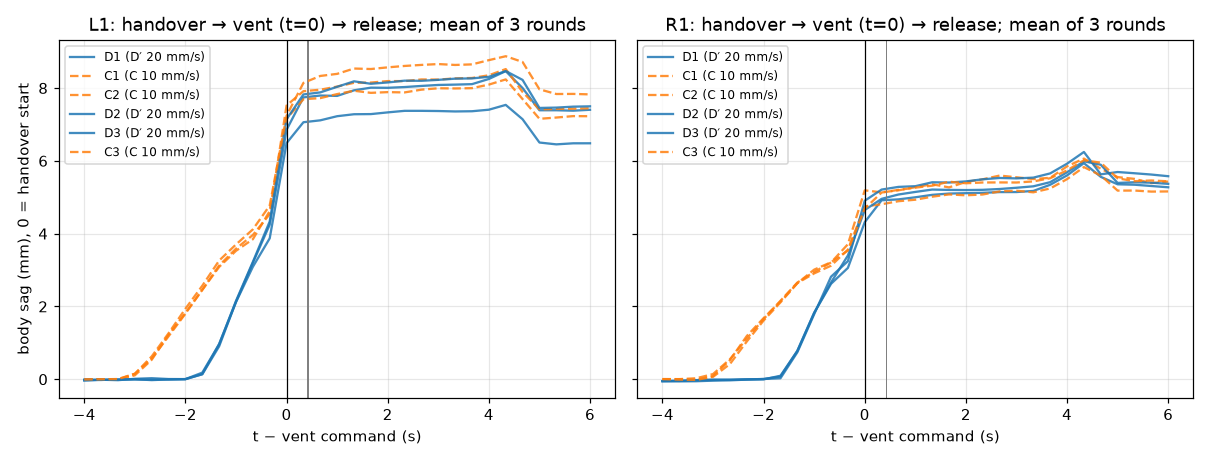
\includegraphics[width=\linewidth]{figures/dprime_profile.png}
\caption{The discrimination result, seen directly: handover profiles
of all six runs aligned on the vent command ($t{=}0$), per-leg means
over rounds (left L1, right R1). At double laying rate (D$'$, solid)
the descent ramp is twice as steep as the control (C, dashed) but ends
at the \emph{same} plateau---the descent tracks laid millimeters, not
elapsed time. \TODO{restyle to match the other figures (fonts/colors);
currently the analysis-report rendering}.}
\label{fig:dprime}
\end{figure}

\subsection{Cost}
\label{sec:cost}

The handover converts an impulsive loss into sustained servo load:
current increase over a run rises from $+0.97\pm0.02$\,A (A) to
$+2.40\pm0.08$\,A (B), which the weights claw back to $+1.85\pm0.08$\,A
(C, $-23\%$ vs.\ B---direction and roughly two-thirds of the modeled
$-32\%$ stored-energy dilution). Cycle time grows by the laying
duration ($2.2$--$3.3$\,s per step at $10$\,mm/s). Both costs are the
explicit price of zero sensing; Sec.~\ref{sec:discussion} argues the
trade.

\subsection{Deviations and threats to validity}
\label{sec:deviations}

We record all deviations. (i)~One run's video started late, cropping
the time-sync marker; the initial rescue (periodic-comb step
regression) locked one tooth off and mis-attributed per-leg slip; the
error was caught by physical implausibility of the per-leg pattern,
re-synchronized by a crop-tolerant marker fit ($R^2=0.99$, amplitude
independently matching the other eight markers), and the corrected run
agrees with all cross-checks. Lesson embedded in the pipeline: check
comb periodicity before step-based sync; the $60$\,s pre-run settle is
now built into the launch sequence. (ii)~The camera moved between two
sessions (never within one); metric scale is per-run by design, and
in-run drift is compensated by the static reference
(${\le}4.4$\,px). (iii)~Battery was not recharged between runs within a
session ($7.5$--$8.1$\,V range); the Latin square decouples it from
condition. (iv)~NCC template score medians ($0.39$--$0.86$) fall below
our internal $0.8$ bar in tilted-board runs; the reference-patch score
($\ge0.988$) and nine-run cross-consistency (CV $1.6$--$4\%$) bound
the impact. (v)~Scale is referenced to the robot-mounted board plane;
top/bottom-edge disagreement ($0.2$--$1.9\%$) bounds the residual
perspective error. (vi)~Segment boundaries at $\pm0.3$\,s move
${\sim}1$\,mm between adjacent columns in two runs (relaxation tails);
merged segments and totals are unaffected. None of these approaches the
order of the effects ($43$--$88\%$).

% =========================================================================
\section{Discussion}
\label{sec:discussion}

\emph{Is this just repairing a badly built robot?} The compliance is
not a construction accident to be engineered away: lightweight printed
legs, bellows cups, and unsensed gear trains are how sub-3\,kg climbers
are built at all, and every element of the failure
combination---compliant support chains, rupture-type detachment,
position-domain actuation---recurs across the platform class
(Sec.~\ref{sec:related}). What the analysis adds beyond the fix is a
design rule: compensability is bounded by the support set's stiffness
profile. The redistribution term \eqref{eq:redistribution} vanishes
under no weighting for the stiffest leg (L1's residual coefficient is
$0.019$ but cannot reach zero)---so a designer who wants software-only
detachment management should bound the \emph{spread} of leg stiffnesses,
not just their level. Conversely, because the remedy is a
${\sim}200$-line, zero-hardware retrofit, it is deployable on the
installed base of position-controlled climbers as-is.

\emph{Why open loop, when the bus current plainly sees the load?} We
argued this choice from data rather than taste. Whole-robot current
cannot be attributed per leg: during a stiff-leg handover the total
shows a plateau whose onset is the balance point of unload/load gains,
not the zero-force point (the leg still bounced $6.9$\,mm at a dose
that ``looked'' converged); during a soft-leg handover the total rises
monotonically---there is no signal to servo on. Per-leg force sensing
is exactly the hardware bill we set out to avoid; motor-current force
estimation \cite{wahrburg2018motor} needs friction models hobby gear
trains do not honor. Meanwhile the open-loop table is estimation-free,
tuning-free, and---as the $n{=}3$ spread shows (relative effects within
$3$ points across replications)---stable across days without
re-calibration. The natural closed-loop upgrade is event-based, not
continuous: the current step at the rupture instant (and ultimately an
IMU pulse) is proportional to residual stored energy and would let the
robot re-trim its own $\delta$ table between climbs; we deliberately
leave this as future work so that the present result stands on zero
sensing.

\emph{Model-gated experiment selection.} The fitted model vetoed one of
our own planned conditions: stiffness-aware shares (choosing $w_i$ to
zero \eqref{eq:redistribution} per leg) move only the redistribution
term, worth $3$--$4$\,mm---not a wall experiment. It also priced the
rate intervention correctly and pre-committed both interpretations. We
found this discipline---models must state their number before the robot
climbs---as valuable as any single result.

\emph{Generalization and limits.} The phenomenon needs three
ingredients: series compliance between anchor and body, detachment that
releases the contact faster than the support can re-equilibrate, and
actuation that tracks position, not force. Vacuum cups on any smooth
surface qualify; directional dry adhesion largely does not (peel-by-design
releases at near-zero force \cite{autumn2006frictional,kim2008smooth}),
which is why the gecko lineage never needed this letter. Our evidence
is one platform, one surface, an in-place proxy task, three rounds, and
$n{=}3$: the effects are huge and internally consistent, but absolute
stiffness (a hang-weight calibration), net-advance climbing with the
handover engaged, longer runs (round-growth factors $\gamma,\beta'$
unsaturated at $r{=}3$), and the micro-mechanism of $\kappa$
(share-concentration vs.\ cup freshness, separable by a
share-perturbation experiment) remain open
\TODO{fold in T4a/T4b results when available}. The $\delta$ table is an
open-loop calibration: payload or posture changes outside the
calibrated regime require re-running the three-dose procedure (one
session) or the event-based re-trim above.

% =========================================================================
\section{Conclusion}

Every discrete-gait suction climber pays a tax at the moment its seals
break. On a compliant, position-controlled hexapod we measured the tax
precisely---$93\%$ of a $64$\,mm/cycle in-place descent concentrated
into post-rupture milliseconds---traced it to elastic energy stored by
the robot's own weight in its leg chains, and showed that the intuitive
remedy (vent slower) cannot work even in principle. Because attached
feet cannot slip, the cure fits in the command stream: return each
leg's stored deflection before venting it, hand the load to the
remaining legs under mean-invariant, rotation-weighted shares, and the
seal breaks with nothing to release. With zero sensors, zero new
hardware, and one offline calibration, the ratchet's rupture component
falls by $88\%$ and the total by $61\%$; what remains obeys a clean
per-millimeter transfer law whose coefficient is set by load-share
allocation---the lever we pull next.

% =========================================================================
\section*{Multimedia}
\TODO{Attachment video (mandatory for this venue): A-vs-C side-by-side
in-place runs $+$ 30\,fps slow-motion of a single rupture; source MOVs
frozen on the lab machine; $\le$20\,MB/180\,s if repurposed for
conference submission.}

\section*{Data Availability}
\TODO{Release bundle: nine $+$ six run logs, trajectories and
decomposition reports, 188 verification crops, analysis pipeline
(tracking, sync, decomposition, fitting), and the $\delta$-calibration
protocol. Decide host (repo/Zenodo) and license.}

\bibliographystyle{IEEEtran}
\bibliography{refs}

\end{document}
